% !TEX root = EIMW2021.tex

\section{The decline in wage inequality in Brazil\label{SECTION: Data}}

\subsection{Data}

Our main data source is an administrative linked employer-employee data set that covers nearly the universe of formal sector workers between 1985 and 2014, called \emph{Rela{\c{c}}{\~{a}}o Anual de Informa{\c{c}}{\~{o}}es Sociais} (RAIS). It consists of annual employment records, which employers are required to report to the Ministry of the Economy (formerly the Ministry of Labor), and allows tracking workers across employers over time.%
%
\footnote{All of our analysis is at the level of the establishment, which we interchangeably refer to as the firm or the employer.} %
%
Our analysis also exploits two household surveys: the \emph{Pesquisa Nacional por Amostra de Domic{\'{i}}lios} (PNAD) and the \emph{Pesquisa Mensal de Emprego} (PME). PNAD is a nationally representative household survey that covers all individuals, regardless of labor market status, in repeated cross sections between 1996 and 2012. PME is a longitudinal household survey that tracks individuals in a rotating monthly panel structure similar to the CPS in the U.S. It covers Brazil's six largest metropolitan regions between 2002 and 2012. Appendix \ref{subsec:Dataset-description} discusses the three datasetes in more detail.

\paragraph{Variables and sample selection.}

RAIS contains the start and end dates of all formal job spells during a given calendar year. We use as our income concept in RAIS the mean monthly earnings in multiples of the current minimum wage---henceforth referred to as wages. These are consistently reported over the period from 1985 to 2014. RAIS also contains unique individual and employer identifiers, gender, age, educational attainment, contractual weekly work hours, and six-digit occupation codes.%

An important difference between the two household surveys, PNAD and PME, in comparison to RAIS is that they do not contain employer identifiers. Instead, they ask respondents questions about the job they held during a reference week preceding the interview, including their work status. Following \citet{MeghirNarita2015}, we classify as informal all self-employed and those in remunerated employment without an official work permit.

For our empirical analysis, we restrict attention to male workers between the ages of 18 and 54. We exclude women and individuals outside of this age range to focus on a subpopulation that is relatively attached to the (formal) labor market.%
%
\footnote{For a separate study of men and women in Brazil's labor market, see \citet{MorchioMoser2020}.} %
%
Among this subpopulation in RAIS, we restrict attention to the largest leave-one-out connected set of workers and firms as in \citet*[][henceforth KSS]{KlineSaggioSolvsten2020}. A connected set is defined as a set of all workers and firms that are linked through worker mobility across firms during a given time period. A leave-one-out connected set is a connected set that remains connected when eliminating worker-firm matches one at a time. No such restriction is necessary or possible in PNAD or PME.%
%
\footnote{The PME is the same data source as used in \citet{MeghirNarita2015}, though we apply slightly different selection criteria (e.g., age 18 to 54 instead of age 23 to 65), use a longer period (from 2002 to 2012 instead of from 2002 to 2007), and measure employment transitions slightly differently (counting any month-to-month transition over the 16-months rotating panel instead of counting months until the first transition or until four months without transition have passed).} %
%


\paragraph{Summary statistics.}

Table \ref{TABLE: summary statistics} summarizes our sample from the three datasets.%
%
\footnote{Additional summary statistics are presented in Appendix \ref{subsec:Summary-statistics}.} %
%
The RAIS data show that between 1996 and 2018, Brazil experienced a 29 log points increase in mean formal sector wages at the same time that there was a striking fall in inequality, with the standard deviation of wages declining by 19 log points. While the age distribution remained somewhat stable, there was a significant increase in educational attainment over this period. Using the PNAD survey data, we find congruent trends in the formal sector wage distribution. Relative to the formal sector, informal wages are initially characterized by lower levels but similar relative dispersion. Throughout 2012, the informal sector wage distribution saw an increase in its mean accompanied by mild compression. At the same time, the employment rate remained stable while the formal employment share rose by eight percentage points. Consistent with the increase in formality, the longitudinal PME data show a rise in the flow rate from formal into formal employment and a decline in the flow rate from formal into informal jobs.%
%
\footnote{In Appendix \ref{app_subsec:sample_selection_size}, we show that official labor force statistics are compatible with the sample sizes in the RAIS.} %
%

\begin{table}[!htb]
  %
  \centering
  \caption{Summary statistics for three datasets, 1996 and 2018\label{TABLE: summary statistics}}
  %
  \pretabvspace
  %
  \begin{tabular}{lccccc}
\multicolumn{1}{c}{} &  &  &  &  & \tabularnewline
\hline
\hline
 & Mean  & St.d. &  & Mean  & St.d. \tabularnewline
\hline
\emph{Panel A. Administrative linked employer-employee data (RAIS)} & \multicolumn{2}{c}{1996} &  & \multicolumn{2}{c}{2018}\tabularnewline
\cline{2-3} \cline{3-3} \cline{5-6} \cline{6-6}
Age  & 32.74 & 9.30 &  & 34.71  & 9.57\tabularnewline
Years of education  & 8.90 & 3.92 &  & 11.06 & 2.93\tabularnewline
Real wage (log real BRL)  & 7.31 & 0.86 &  & 7.60 & 0.67\tabularnewline
Observations (millions)  & 17.20 &  &  & 27.60 & \tabularnewline
 &  &  &  &  & \tabularnewline
\emph{Panel B. Cross-sectional household survey data (PNAD)} & \multicolumn{2}{c}{1996} &  & \multicolumn{2}{c}{2012}\tabularnewline
\cline{2-3} \cline{3-3} \cline{5-6} \cline{6-6}
Real wage (log real BRL, formal sector)  & 7.01 & 0.81  &  & 7.13  & 0.62\tabularnewline
Real wage (log real BRL, informal sector)  & 6.26  & 0.81  &  & 6.56  & 0.78\tabularnewline
Employment rate  & 0.95  &  &  & 0.95  & \tabularnewline
Formal employment share  & 0.68  &  &  & 0.76  & \tabularnewline
Observations (thousands)  & 74.5  &  &  & 86.0  & \tabularnewline
 &  &  &  &  & \tabularnewline
\emph{Panel C. Longitudinal household survey data (PME)} & \multicolumn{2}{c}{2002} &  & \multicolumn{2}{c}{2012}\tabularnewline
\cline{2-3} \cline{3-3} \cline{5-6} \cline{6-6}
Transition rate nonemployed-employed  & 0.08  &  &  & 0.10  & \tabularnewline
Transition rate employed-nonemployed  & 0.05  &  &  & 0.04  & \tabularnewline
Observations (thousands)  & 94.3  &  &  & 121.2  & \tabularnewline
\hline
\end{tabular}

  %
  \posttabvspace
  %
  \begin{minipage}[t]{1\columnwidth}%
    \begin{spacing}{0.75}
      \emph{\scriptsize{}Notes: }{\scriptsize{}Years of education are set to 0 for illiterate, 3 for some primary school, 5 for primary school, 7.5 for some middle school, 9 for middle school, 11 for some high school, 12 for high school, 14 for some college, and 16 for at least a bachelor's degree. Real wage refers to mean actual (in RAIS) or usual (in PNAD) monthly earnings in constant December 2018 BRL. Employment comprises domestic workers, employees, and self-employed. Formal employment is employment with a legal work permit. Monthly transition rates are between employment (i.e., formal employment) and nonemployment (i.e., informal employment + unemployment). %
      \emph{\scriptsize{}Source: } RAIS, 1996 and 2018, PNAD, 1996 and 2012, and PME, 2002 and 2012.}
    \end{spacing}
  \end{minipage}
  %
\end{table}


Panels \subref{fig:histograms_log_1996_2018_A} and \subref{fig:histograms_log_1996_2018_B} of Figure \ref{fig:histograms_log_1996_2018} show histograms of log wages in 1996 and 2018, respectively. Evidently, Brazil's inequality decline was associated with relatively greater compression in the left tail of the wage distribution over this period. Indeed, panel \subref{fig:histograms_log_1996_2018_C} shows that lower-tail wage inequality---as measured by the P50/P10 log wage percentile ratio---fell by significantly more compared to upper-tail inequality---as measured by the P90/P50 log wage percentile ratio. While both tails of the wage distribution experienced some compression, lower-tail inequality fell by almost 40 percent between 1996 and 2018, while upper-tail inequality fell by around 15 percent over the same period.


\begin{figure}[!htb]
  %
  \centering
  \caption{\label{fig:histograms_log_1996_2018}Lower- and upper-tail inequality}
  %
  \prefigvspace
  %
  \subfloat[Histogram of log wages, 1996\label{fig:histograms_log_1996_2018_A}]{%
   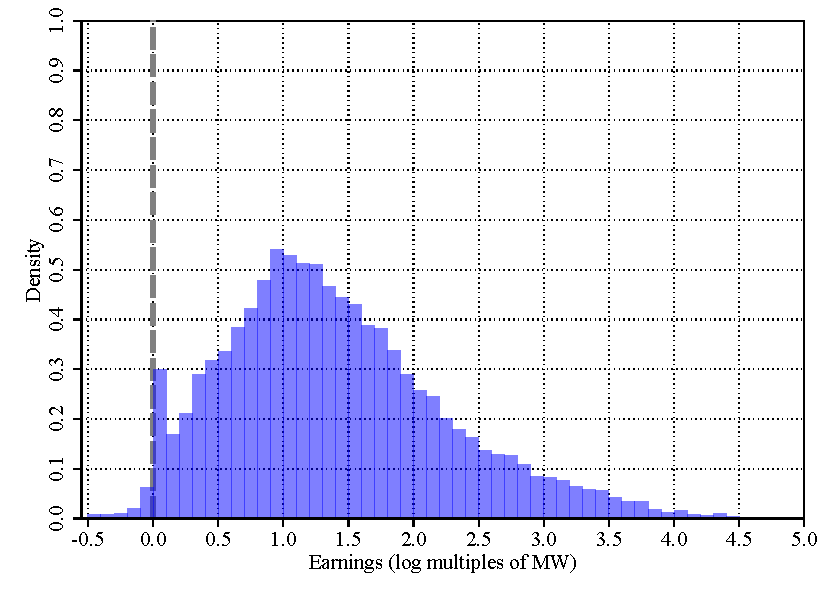
\includegraphics[width=0.33\columnwidth]{_figures/fig1A.pdf}% _figures/hist_spike_ln_1996.pdf
    %
  }
  \subfloat[Histogram of log wages, 2018\label{fig:histograms_log_1996_2018_B}]{%
   \includegraphics[width=0.33\columnwidth]{_figures/fig1B.pdf}% _figures/hist_spike_ln_2018.pdf
    %
  }
  \subfloat[Percentile ratios, 1996--2018\label{fig:histograms_log_1996_2018_C}]{%
   \includegraphics[width=0.33\columnwidth]{_figures/fig1C.pdf}% _figures/inc_p50_p10_inc_p90_p50_short.pdf
    %
  }%
  \\
  %
  \postfigvspace
  %
  \begin{minipage}[t]{1\columnwidth}%
    \begin{spacing}{0.75}
      \emph{\scriptsize{}Notes: }{\scriptsize{}Panels \subref{fig:histograms_log_1996_2018_A} and \subref{fig:histograms_log_1996_2018_B} show histograms of log wages in multiples of the current minimum wage based on 60 equi-spaced bins for population of male workers aged 18--54 for 1996 and 2018, respectively. Panel \subref{fig:histograms_log_1996_2018_C} plots lower- and upper-tail wage inequality, as measured by the P50/P10 and the P90/P50 log wage percentile ratios between 1996 and 2018, normalized to $1.0$ in 1996. %
      \emph{\scriptsize{}Source: } RAIS, 1996--2018.}
    \end{spacing}
  \end{minipage}
  %
\end{figure}




\subsection{Dissecting Brazil's decline in earnings inequality: The role of firms\label{subsec:Motivating-facts}}

To understand the decline in wage inequality in Brazil, we follow \citet{ABEM2018} in implementing a statistical decomposition of wages among formal sector workers in Brazil. Motivated by the fact that a large share of empirical wage dispersion is within detailed worker groups based on observable characteristics---as demonstrated in Appendix \ref{app_subsec:unobserved_heterogeneity}---we estimate two-way fixed effect specifications based on the econometric framework by AKM. The goal of the exercise is to assess whether firms are a key channel through which the distribution of wages may change over time, either through adjustments in firm pay policies or through worker reallocation across firms. Specifically, we decompose log wages $w_{ijt}$ of individual $i$ working at firm $j$ in year $t$ within five-year periods as
%
\begin{equation}
  w_{ijt}=\alpha_{i}+\psi_{j} + X_{it}\beta +\varepsilon_{ijt},\label{eq: AKM framework}
\end{equation}
%
where $\alpha_{i}$ denotes a worker fixed effect, $\psi_{j}$ denotes a firm fixed effect, $X_{it}$ is a vector of time-varying worker characteristics---including education-specific age dummies restricted to be flat between ages 45 and 49, education-specific year dummies, contractual work hours dummies, and six-digit occupation dummies---and $\varepsilon_{ijt}$ is a residual satisfying a strict exogeneity condition. %
%
Equation \eqref{eq: AKM framework} is identified off workers switching employers within the largest set of firms connected through worker mobility. While ordinary least squares (OLS) estimates of individual coefficients in equation \eqref{eq: AKM framework} are unbiased, the variance and covariance terms based on these coefficients generally are biased in finite samples. To correct for this bias, we adopt the leave-one-out estimator developed by KSS, which yields unbiased estimates of the variance components of log wages based on equation \eqref{eq: AKM framework}.%
%
\footnote{There has been a fruitful debate around the benefits and drawbacks of estimating AKM wage equations, including \citet{Andrews2008}, \citet{EeckhoutKircher2011}, \citet{Lopesdemelo2016}, \citet{Card2018}, \citet{BonhommeLamadonManresa2019}, \citet{BonhommeHolzheuLamadonManresaMogstadSetzler2020}, and \citet{Borovickova2020}. In related work, \citet{ABEM2018} and \citet{GerardLagosSeverniniCard2020} present a battery of robustness checks, which suggest that the AKM equation is well suited for describing the Brazilian data during this period.} %
%

Table \ref{TABLE: AKM summary statistics} presents a decomposition of the variance of log wages based on the AKM wage equation \eqref{eq: AKM framework}, separately for a five-year period centered around 1996 (i.e., from 1994--1998) and a five-year period ending in 2018 (i.e., from 2014--2018). For each period, we report results from four estimations: %
%
one without KSS correction and without controls in columns (1) and (5), %
one with KSS correction and without controls in columns (2) and (6), %
one without KSS correction and with controls in columns (3) and (7), and %
one with KSS correction and with controls in columns (4) and (8). %
%
The last four columns report the change between periods for each of the four sets of estimates.

\begin{table}[!htb]
  %
  \centering
  \caption{\label{TABLE: AKM summary statistics}Decomposition of the variance of log wages over time}%
  %
  \pretabvspace
  %
  \resizebox{\textwidth}{!}{%
  \begin{tabular}{lcccccccccccccc}
  \multicolumn{2}{c}{} &  &  &  &  &  &  &  &  &  &  &  &  & \tabularnewline
  \hline
  \hline
   & \multicolumn{4}{c}{Variance (\%), 1994--1998} &  & \multicolumn{4}{c}{Variance (\%), 2014--2018} &  & \multicolumn{4}{c}{Change (\%), 1994--1998 to 2014--2018}\tabularnewline
  \hline
   & (1)  & (2)  & (3)  & (4)  &  & (5)  & (6)  & (7)  & (8)  &  & (5)$-$(1)  & (6)$-$(2)  & (7)$-$(3)  & (8)$-$(4)\tabularnewline
  \hline
  \multicolumn{1}{l}{$Var(w_{ijt})$} & 0.709  & 0.709  & 0.709  & 0.709  &  & 0.444 & 0.444 & 0.444 & 0.444 &  & -0.265 & -0.265 & -0.265 & -0.265\tabularnewline
   & (100\%)  & (100\%)  & (100\%)  & (100\%)  &  & (100\%)  & (100\%)  & (100\%)  & (100\%)  &  & (100\%) & (100\%) & (100\%) & (100\%)\tabularnewline
  $Var(\hat{\alpha}_{i})$  & 0.323  & 0.279  & 0.217  & 0.176  &  & 0.264 & 0.241 & 0.173 & 0.154 &  & -0.059 & -0.038 & -0.044 & -0.022\tabularnewline
   & (46\%)  & (39\%)  & (31\%)  & (25\%)  &  & (59\%) & (54\%) & (39\%) & (35\%) &  & (22\%) & (14\%) & (17\%) & (8\%)\tabularnewline
  $Var(\hat{\psi}_{j})$  & 0.212  & 0.198  & 0.201  & 0.187  &  & 0.083 & 0.076 & 0.078 & 0.072 &  & -0.129 & -0.122 & -0.123 & -0.115\tabularnewline
   & (30\%)  & (28\%)  & (28\%)  & (26\%)  &  & (19\%) & (17\%) & (18\%) & (16\%) &  & (49\%) & (46\%) & (46\%) & (43\%)\tabularnewline
  $2\times Cov(\hat{\alpha}_{i},\hat{\psi}_{j})$  & 0.140  & 0.163  & 0.098  & 0.120  &  & 0.081 & 0.092 & 0.061 & 0.070 &  & -0.059 & -0.071 & -0.037 & -0.050\tabularnewline
   & (20\%)  & (23\%)  & (14\%)  & (17\%)  &  & (18\%) & (21\%) & (14\%) & (16\%) &  & (22\%) & (27\%) & (14\%) & (19\%)\tabularnewline
  $Var(\hat{\varepsilon}_{ijt})$  & 0.034  & 0.070  & 0.033  &  &  & 0.017 & 0.036 & 0.016 &  &  & -0.017 & -0.034 & -0.017 & \tabularnewline
   & (5\%)  & (10\%)  & (5\%)  &  &  & (4\%) & (8\%) & (4\%) &  &  & (6\%) & (13\%) & (6\%) & \tabularnewline
   &  &  &  &  &  &  &  &  &  &  &  &  &  & \tabularnewline
  $Corr\left(\hat{\alpha_{i}},\hat{\psi_{j}}\right)$  & 0.267  & 0.347  & 0.234  & 0.330  &  & 0.273 & 0.340 & 0.263 & 0.332 &  &  &  &  & \tabularnewline
   &  &  &  &  &  &  &  &  &  &  &  &  &  & \tabularnewline
  $R^{2}$  & 0.951  & 0.902  & 0.953  &  &  & 0.961 & 0.919 & 0.965 &  &  &  &  &  & \tabularnewline
  Obs. (mm)  & 67.8  & 67.8  & 67.8  & 67.8  &  & 131.9 & 131.9 & 131.9 & 131.9 &  &  &  &  & \tabularnewline
   &  &  &  &  &  &  &  &  &  &  &  &  &  & \tabularnewline
  KSS correction  & No  & Yes  & No   & Yes  &  & No  & Yes  & No   & Yes  &  & No  & Yes  & No   & Yes\tabularnewline
  Controls        & No  & No   & Yes  & Yes  &  & No  & No   & Yes  & Yes  &  & No  & No   & Yes  & Yes\tabularnewline
  \hline
  \end{tabular}
}

  %
  \posttabvspace
  %
  \begin{minipage}[t]{1\columnwidth}%
    \begin{spacing}{0.75}
      \emph{\scriptsize{}Notes: }{\scriptsize{}This table shows plug-in and bias-corrected variance components of log wages based on estimating AKM equation \eqref{eq: AKM framework} for the population of male workers of age 18--54 in 1994--1998 and 2014--2018. $Var(w_{ijt})$ denotes the variance of log wages, $Var(\hat{\alpha}_{i})$ denotes the variance of estimated person fixed effects, $Var(\hat{\psi}_{j})$ denotes the variance of estimated firm fixed effects, $2\times Cov(\hat{\alpha}_{i},\hat{\psi}_{j})$ denotes two times the sum of the covariance between estimated person fixed effects $\hat{\alpha}_{i}$ and estimated firm fixed effects $\hat{\psi}_{j}$, and $Var(\hat{\varepsilon}_{ijt})$ denotes the variance of estimated residuals. For columns (3)--(4) and (7)--(8), omitted terms include the variance of the estimated component of log wages due to observable worker characteristics, $Var(X_{it}\hat{\beta})$, and two times the sum of covariance terms involving observable worker characteristics. $Corr\left(\hat{\alpha_{i}},\hat{\psi_{j}}\right)$ denotes the correlation between estimated person fixed effects $\alpha_{i}$ and estimated firm fixed effects $\psi_{j}$. Variance shares are in parentheses in columns (1)--(8). Share of total change in the variance of log wages is in parentheses in the last four columns. Observations are in millions of worker-years. KSS correction refers to leave-one-out estimators of variance components by \citet{KlineSaggioSolvsten2020}. The variance of estimated residuals, $Var(\hat{\varepsilon}_{ijt})$, and the coefficient of determination, $R^2$, are not reported in columns (4) and (8) due to their omission in the KSS leave-one-out estimation with controls. Controls include education-specific age dummies restricted to be flat between ages 45 and 49, education-specific year dummies, contractual work hours dummies, and occupation dummies. %
      \emph{\scriptsize{}Source:} RAIS, 1994--1998 and 2014--2018.}
    \end{spacing}
  \end{minipage}
  %
\end{table}

During 1994--1998 (columns 1--4), out of the total variance of wages of 70.9 log points, between 46 and 25 percent are attributable to the variance of person fixed effects. The inclusion of worker controls reduces this share by around one third, while the KSS correction further reduces it. Between 30 percent (column 1) and 26 percent (column 4) of the total variance of log wages are attributed to the firm pay component, with little variation in this share with and without KSS correction or controls. There is significant positive worker-firm sorting, as measured by the correlation between worker and firm fixed effects of 0.330 including the KSS correction and controls. The associated value of two times their covariance term equals 0.120, which accounts for an additional 17 percent of the total variance (column 4).

During 2014--2018 (columns 5--8), the total variance of wages is 44.4 log points, which is 26.5 log points lower relative to 1994--1998. While worker heterogeneity is the most important factor behind the cross-sectional wage variance, a drop in the variance of firm fixed effects constitutes between 49 percent (comparing columns 5 and 1) and 43 percent (comparing columns 8 and 4) of the total decline. A lower variance of person fixed effects accounts for between 22 percent (comparing columns 5 and 1) and 8 percent (comparing columns 8 and 4) of the total decline. Lower covariance terms and residual variance account for the remaining decline. Between the two periods, the correlation between worker and firm fixed effects remained roughly constant, as did the coefficient of determination for the reported specifications.

In summary, Brazil saw a remarkable decline in wage inequality between 1996 and 2018, which was partly driven by a reduction in pay differences across firms for identical workers. We interpret this as evidence for the hypothesis that the decline in inequality over this period was the result of changes in firms' pay policies rather than solely due to changes in worker composition.
